\documentclass[12pt,letterpaper]{article}

\usepackage{graphicx}                 %Include the graphix package
\usepackage{aas_macros}               %Include Journal Abbrev.
\usepackage[margin=1in]{geometry}     % Set page geometry

\setlength{\parindent}{0pt}  % Do not indent beginning of paragraphs
\setlength{\parskip}{12pt}   % Space between paragraphs

\title{Contractual Obligation Paper}
\author{Tricia McMillan}
\date{\today}

\begin{document}

\maketitle

\section{Some Text}

This is some text. Some of the text is \textit{set in italics} and some
is \textbf{set in bold}. The author is visiting from the Sirius
Cybernetics Corporation where she holds the post of Professor of Vogon
poetry\cite{adams1979hitchhiker}. Professor McMillan is currently
researching adapting the Moon as a concert
venue\cite{2011JGRE..11600H03S}.

This is an equation $\nabla \cdot B = 0$ in the middle of a line.

This is an equation on it own line: 

\[
 \nabla \cdot D = \rho
\]

This is an equation on its own line with an equation number:

\begin{equation}
    \nabla \times H = J + \frac{\partial D}{\partial t}
\end{equation}

This seems like a good place to put a table. 

\begin{table}[h]
\centering
\begin{tabular}{ccl}
{\it X} & {\it Y} & A Comment \\ \hline
1.2 & 2.3 & Another Comment\\
3.4 & 4.5 & Yet Another Comment\\ \hline
\end{tabular}
\caption{This is a Table}
\label{ATable}
\end{table}

\subsection{More Stuff}

\LaTeX\ has its own idea about where tables and figure go. Sometimes
it will place them where you want and sometimes it will decide it does
not like what you want and will place them where it thinks it is best.
Do not worry about it.

\begin{figure}[h]
\begin{center}
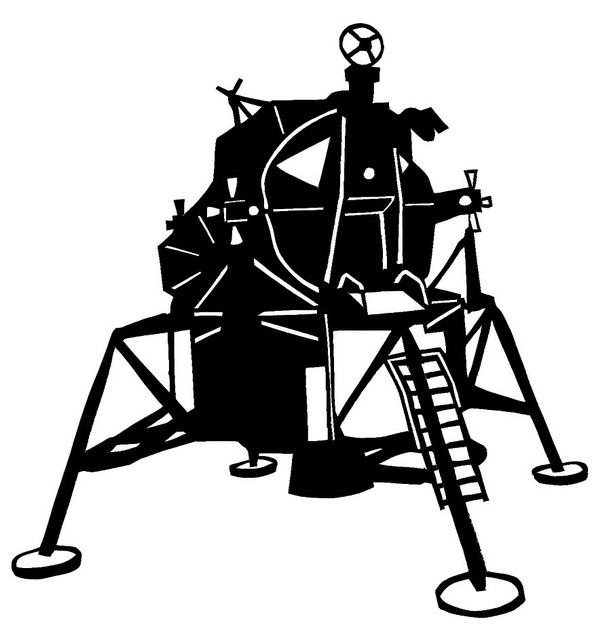
\includegraphics[width=2cm]{LM.jpg}
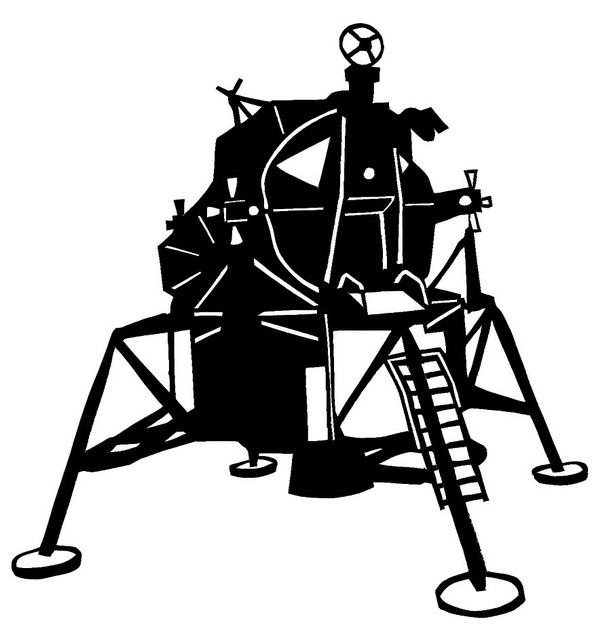
\includegraphics[width=4cm]{LM.jpg}
\caption{A couple of figures with a common caption.}
\label{TwoFigs}
\end{center}
\end{figure}

\begin{figure}[h]
\begin{center}
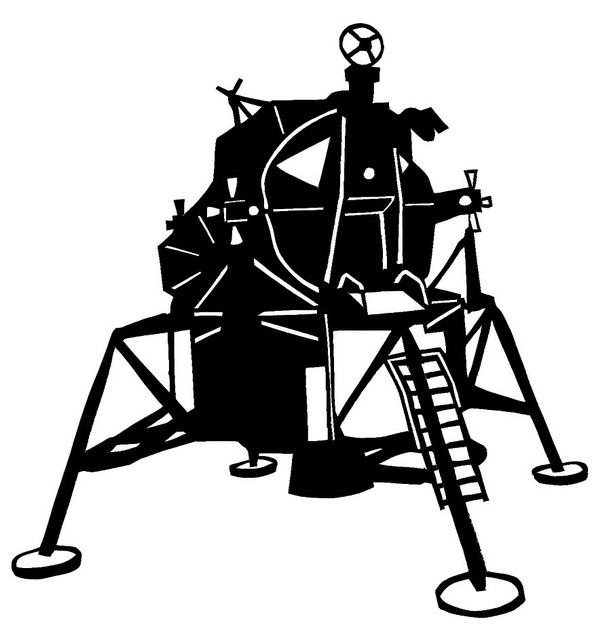
\includegraphics[width=4cm,angle=180]{LM.jpg}
\caption{A single figure (upside down).}
\label{SingleFig}
\end{center}
\end{figure}

Here is a final bit of text referencing Figure \ref{SingleFig} and Table
\ref{ATable}.

% BIBLIOGRAPHY

\bibliographystyle{unsrt}
\bibliography{MyRefs}

\end{document}
